% ========================================================================
% Adaptação do modelo de artigo para a Revista Brasileira de Criminalística
% Versão 0.8
% Adelino Pinheiro Silva- adelinocpp@yahoo.com
% ========================================================================

% === DECLARAÇÃO DO TIPO DE DOCUMENTO ====================================
\documentclass{RBClatex}
% ========================================================================
\graphicspath{{Figuras/}}


% === Instruções Gerais ==================================================
% Antes de mais nada:
% Utilize codificação UTF-8
		
% === Definições para revisão ============================================
% Para garantir a revisão duplo cega é importante suprimir, do arquivo em 
% .pdf, e possivelmente do arquivo .tex, qualquer referência que pode identificar 
% os autores
% Trechos para esta substituição estão sugeridos nos comentários
% --- ATENCAO PARA AS VARIAVEIS ABAIXO -----------------------------------
\providetoggle{TextoEmRevisao}  
\settoggle{TextoEmRevisao}{true} 
% Enquanto  a variável TextoEmRevisao for true o texto terá configuraçẽos 
% de revisão, quando setar para false 
% \settoggle{TextoEmRevisao}{false}
% o texto vai adotar algumas configurações de trabalho final. Neste momento
% as variaveis abaixo devem estar corretamente preenchidas:
% Observação: Preencha apenas a página inicial, a final é automática
\def\VOLUME/{0}
\def\NUMERO/{0}
\def\PAGINICIAL/{0}
\def\PAGFINAL/{\pageref*{LastPage}}
\def\ANO/{2000}
\def\DOI/{http://dx.doi.org/10.15260/rbc.v0i0.00}
\def\DATARECEBIDO/{00/00/2000}
\def\DATAREVISADO/{00/00/20000}
\def\DATAACEITO/{00/00/2000}
% ========================================================================


% ========================================================================

% === INFORMAÇÕES DO ARTIGO ==============================================

% --- Título -------------------------------------------------------------
% Digite o título no campo abaixo logo após o comando "\selectfont{" \vspace{-2mm}}
% e antes do comando "\vspace{-2mm}}"
% Não há restrição de caracteres e 
\title{\fontsize{17}{20.4}\selectfont{Título pleno do artigo: não devendo exceder 25 palavras \vspace{-2mm}}}

% ------------------------------------------------------------------------
% -- Lista de autores e afiliação ----------------------------------------
% - Não abreviar o nome de citação (último nome em regra geral).
% - O autor principal (ou único autor) deve ser seguido pelo comando "\footnote{First  Author}"
% para gerar a abreviatura do cabeçalho.
% - As afiliações são enumeradas por letras minúsculas 
% - O asterisco "*" indica o endereço eletrico de correspondência
% - A última afiliação deve ser seguida do comando "\vspace{1.75mm}"
% - A afiliação "*" é o endereço de correspondência
% - No endereço para correspondência o campo \href{mailto: } deve conter o 
% e-mail, exemplo "\href{mailto:adelinocpp@gmail.com}". Já no campo "\uline{ }"
% a forma como ele é apresentado no texto. Exemplo: \uline{suporte\_rbc@gmail.com}.
% cuidado com e-mail com caracteres especiais (no exemplo "_" deve ser 
% inserido como "\_"). Em caso de dúvidas consulte a lista de caracteres 
% especiais: https://en.wikibooks.org/wiki/LaTeX/Special_Characters
%\iftoggle{TextoEmRevisao}
%{
%% ------------------------------------------------------------------------
%% --- SUGESTÃO DE AUTOR PARA REVISÃO DUPLO CEGA --------------------------
%% ------------------------------------------------------------------------
% Descomente as linhas a seguir e comente (ou melho apague) as linahs com 
% os nomes reais dos autores.
% -------
%\author[a,*]{X.Y. Autor\footnote{First  Author}} % precisa do \footnote{First  Author}
%\affil[a]{Revista Brasileira de Criminalística, Brasília (DF), Brasil \vspace{1.75mm}} 
%\affil[*]{Endereço de e-mail para correspondência: \href{mailto:suporte_rbc@gmail.com}{\uline{suporte\_rbc@gmail.com}} . Tel.: +55-61-3361-0771}
% -------
\author[a,*]{A.P. Silva\footnote{First  Author}} % precisa do \footnote{First  Author}
\author[b]{J.A. Gomes}
\author[b]{C.A. Andrade}
\author[c]{A.T. Oliveira}
\affil[a]{Instituto de Criminalística, Polícia Civil de Minas Gerais, Minas Gerais (MG), Brasil}
\affil[b]{Instituto de Criminalística, Polícia Civil do Distrito Federal, Brasília (DF), Brasil}
\affil[c]{Instituto de Criminalística, Superintendência de Polícia Técnico-Científica, Goiânia (GO), Brasil \vspace{1.75mm}} 
\affil[*]{Endereço de e-mail para correspondência: \href{mailto:adelinocpp@gmail.com}{\uline{adelinocpp@yahoo.com}} . Tel.: +55-31-988013605}
% -------
\date{}
% ------------------------------------------------------------------------

% ------------------------------------------------------------------------
% --- Cabeçário e rodapé -------------------------------------------------
%\makeoddhead{plain}{}{\fontsize{8}{9.2}\selectfont{\vspace{-3.5mm}{\color{red} \authors, Rev. Bras. Crim. 0(0),0-0, 2000}}}{}
%\makeevenhead{plain}{}{\fontsize{8}{9.2}\selectfont{{\vspace{-3.5mm}\color{red} \authors, Rev. Bras. Crim. 0(0),0-0, 2000}}}{}
\iftoggle{TextoEmRevisao}
{
\makeoddhead{plain}{}{\vspace{2.5mm}\FCPreR{ \authors, Rev. Bras. Crim. \textbf{\VOLUME/(\NUMERO/)},\PAGINICIAL/-\PAGFINAL/, \ANO/}}{}
\makeevenhead{plain}{}{\vspace{2.5mm}\FCPreR{\authors, Rev. Bras. Crim. \textbf{\VOLUME/(\NUMERO/)},\PAGINICIAL/-\PAGFINAL/, \ANO/}}{}
}
{
\makeoddhead{plain}{}{\vspace{2.5mm}\FCPosR{ \authors, Rev. Bras. Crim. \textbf{\VOLUME/(\NUMERO/)},\PAGINICIAL/-\PAGFINAL/, \ANO/}}{}
\makeevenhead{plain}{}{\vspace{2.5mm}\FCPosR{\authors, Rev. Bras. Crim. \textbf{\VOLUME/(\NUMERO/)},\PAGINICIAL/-\PAGFINAL/, \ANO/}}{}
}
\makeoddfoot{plain}{}{}{\vspace{0mm}\fontsize{9}{10.8}\selectfont{\thepage}}
\makeevenfoot{plain}{}{}{\vspace{0mm}\fontsize{9}{10.8}\selectfont{\thepage}}
% ========================================================================

% === INÍCIO DO DOCUMENTO ================================================
\begin{document}
\clearpage
\setcounter{page}{\PAGINICIAL/}
% --- Retira espaço extra obsoleto entre as frases -----------------------
\frenchspacing 
% ------------------------------------------------------------------------

\twocolumn[    		% INICIO DE ARTIGO EM DUAS COLUNAS
\begin{@twocolumnfalse}
% --- Definição do grupo que contém a o ISSN, LOGOTIPO, DOI e TÍTULO -----
\begingroup
{
	{
	\begin{addmargin}[3mm]{0mm}
	\iftoggle{TextoEmRevisao}
	{
	\flushleft\FCPreR{v. \VOLUME/, n. \NUMERO/, p. \PAGINICIAL/-\PAGFINAL/, \ANO/ \vspace{-0.3\baselineskip} \break ISSN 2237-9223}
	}
	{
	\flushleft\FCPosR{v. \VOLUME/, n. \NUMERO/, p. \PAGINICIAL/-\PAGFINAL/, \ANO/ \vspace{-0.3\baselineskip} \break ISSN 2237-9223}	
	}
	
	\end{addmargin}
	}
}
\flushright{
	\vspace{-12.00mm}
 
	\includegraphics[keepaspectratio, width=7.73 cm]{RBClogo.pdf} \\ \vspace{-1mm}
	\fontsize{11}{13.2}\selectfont{\textbf{DOI:} \href{\DOI/}{\uline{\DOI/}}}
}
\vspace{-11.00mm}
\let\newpage\relax%
\maketitle

\vspace{-16.5mm}
\iftoggle{TextoEmRevisao}
{
\centering\FCPreR{Recebido em \DATARECEBIDO/; Revisado em \DATAREVISADO/; Aceito em \DATAACEITO/}
}
{
\centering\FCPosR{Recebido em \DATARECEBIDO/; Revisado em \DATAREVISADO/; Aceito em \DATAACEITO/}
}
\vspace{2.75mm}

\noindent\rule{\textwidth}{0.1mm}
\vspace{-7mm}
\endgroup
% ----------------------------------------------

% resumo em português

\renewcommand{\abstractname}{Resumo}
\begin{onecolabstract}

\vspace{-1.5mm}
\noindent
Este documento fornece instruções de formatação para os autores prepararem artigos para publicação na Revista Brasileira de Criminalística utilizando o \textit{template} em \LaTeX. Os autores devem seguir as instruções contidas no documento para os trabalhos serem publicados. Você pode usar esse documento bem como as instruções como um modelo no qual você pode digitar seu texto e ajustar as configurações em \LaTeX. Ressalta-se que o resumo deve apresentar os objetivos, o método utilizado e as principais conclusões, e ter, no máximo: (i) 250 palavras para trabalhos nas categorias: relato de pesquisa, estudo teórico, relato de experiência profissional e revisão crítica de literatura; (ii) 100 palavras para trabalhos nas categorias: comunicação breve, carta ao editor e nota técnica; (iii) as categorias resenha e notícia não admitem resumo.
 
\vspace{6pt}

\noindent
\footnotesize\textit{Palavras-chaves}: Modelo; \LaTeX; ABC; Revista Brasileira de Criminalística; Máximo 5 Palavras-Chave.

\vspace{-2.5mm}
\noindent\rule{\textwidth}{0.1mm}

\end{onecolabstract}
\vspace{-4mm}
\renewcommand{\abstractname}{Abstract}

\begin{onecolabstract}

%	\begin{otherlanguage*}{english}
		\vspace{-1.5mm}
		\noindent
		This document gives formatting instructions for authors preparing papers for publication in the Revista Brasileira de Criminalística using \LaTeX \textit{template}. The authors must follow the instructions given in the document for the papers to be published. You can use this document as both an instruction set and as a \textit{template} into which you can type your own text and adjust settings of \LaTeX. It is emphasized that the abstract should present objectives, methodology and main conclusions, and have no more than: (i) 250 words for the categories: research report, theoretical study, reports of professional experience and critical review of literature, (ii) 100 words for the categories: brief communication, letter to the editor and technical note, (iii) the categories review and news do not allow abstract.
		
		\vspace{6pt}
		
		\noindent
		\footnotesize\textit{Key-words}: Template; \LaTeX; ABC; Revista Brasileira de Criminalística; Maximum 5 Keywords.
		
		\vspace{-2.5mm}
		\noindent\rule{\textwidth}{0.1mm}
%	\end{otherlanguage*}  
\end{onecolabstract}
\vspace{2.5mm}
\end{@twocolumnfalse}
]				% FIM DE ARTIGO EM DUAS COLUNAS
% ---

% ----------------------------------------------------------
% ELEMENTOS TEXTUAIS
% ----------------------------------------------------------
%\textual

% ----------------------------------------------------------
% Introdução
% ----------------------------------------------------------
\section{Introdução}

A Revista Brasileira de Criminalística destina-se a publicação de artigos originais que contribuam para a promoção, a divulgação e o desenvolvimento científico e tecnológico das ciências forenses, referentes aos resultados de pesquisas, avanços e projetos técnico-científicos relacionados à criminalística, incluindo as interfaces com outros ramos da ciência, como Física, Química, Biologia, Odontologia, Farmacologia, Informática, Contabilidade e Engenharias.

A abreviatura do título da revista é \textbf{Rev. Bras. Crim.}, que deve ser usada em referências bibliográficas.
Este documento é um modelo. Uma cópia eletrônica pode ser baixada do site da revista. Para dúvidas sobre as orientações do artigo, entre em contato com a revista.

O texto deve ter uma organização de reconhecimento fácil, sinalizada por um sistema de títulos e subtítulos que reflitam a organização. Este, sempre que possível, deve iniciar com uma Introdução, redigida para o público geral que lê a revista e não para o especialista. Esta seção deve conter a descrição do problema, sua importância, os resultados significativos e as conclusões dos trabalhos anteriores, além dos objetivos do trabalho atual.

As seções nas quais o trabalho possa ser enquadro são as seguintes: 
\begin{itemize}[noitemsep,topsep=0pt,leftmargin=*,labelindent=7.5mm,labelsep=2mm]
	\item Balística forense
	\item Contabilidade forense
	\item Crimes contra a pessoa e contra o patrimônio
	\item Crimes contra o meio ambiente
	\item Criminalística geral
	\item Delitos de trânsito e identificação veicular
	\item Documentoscopia e grafoscopia
	\item Engenharia legal
	\item Entomologia forense
	\item Identificação humana
	\item Informática forense
	\item Laboratório forense
	\item Medicina legal e odontologia forense
	\item Forense Nuclear
	\item Perícia de incêndio e explosão
	\item Perícia em áudio e vídeo e fonética forense 
\end{itemize}

Como trata-se de um \textit{template} em \LaTeX, nas próximas seções serão serão descritas as formas de inserir o texto do artigo no \textit{template} sem se preocupar com a formatação. De certa forma este é um guia das dificuldades do \LaTeX. Mas podem confiar que o ganho é muito maior que o esforço.

Existe uma vasta gama de interfaces de desenvolvimento integrado (IDE) para \LaTeX. Os autores recomendam o TexStudio\footnote{Pode ser obtido em: https://www.texstudio.org/.}.


\section{Formatação da página}

O texto é formatado básicamente pela classe RBClatex, implementada no arquivo RBClatex.cls. No início do arquivos temos a declaração:
\begin{verbatim}
	\documentclass{RBClatex}
\end{verbatim}
que carrega os principais pacotes para redação de artigos e define os parâmetros de formatação como página, margens, fonte, estilo de referências bibliográficas, entre outros.

Isto quer dizer que o presente autor dispôs de tempo e esforço para realizar a formatação do documento. Ficando para os autores dos próximos artigos apenas o esforço de realizar a redação e inserir seus dados. Esta é o primeiro ganho do \LaTeX. O esforço de formatação é realizado apenas uma vez e futuros autores não precisam se preocupar com:
\begin{itemize} [noitemsep,topsep=0pt,leftmargin=*,labelindent=7.5mm,labelsep=2mm]
	\item Layout da Página;
	\item Estilo da página;
	\item Fonte do texto do documento;
	\item Título e detalhes dos autores
	\item Seção de títulos.
\end{itemize}

Apenas deixo a importante regra de que não mais do que dois subtítulos devem ser usados. Em \LaTeX utiliza-se respectivamente os comandos
\begin{verbatim}
	\section{}
	\subsection{}
	\subsubsection{}
\end{verbatim}
para definir seções em nível primário, secundário e terciário (este é o segundo subtítulo).

\subsection{Alguns Comandos e Configurações em \LaTeX}

\subsubsection{Listas}

A principal diferença dos editores da família \TeX e dos editores WYUIWYG (\textit{What You See Is What You Get}) é que toda a formatação é realizada por comando. 

Para criar uma lista de tópicos utilize o comando 
\begin{verbatim}
	\begin{itemize}[noitemsep,topsep=0pt,
	leftmargin=*,labelindent=7.5mm,
	labelsep=2mm]
		\item Tópico 1;
		\item Tópico 2.
	\end{itemize}
\end{verbatim}
que resulta na seguinte lista:
\begin{itemize}[noitemsep,topsep=0pt,leftmargin=*,labelindent=7.5mm,labelsep=2mm]
	\item Tópico 1;
	\item Tópico 2.
\end{itemize}

Nota-se que os comandos \verb|\begin{itemize}| e \verb|\end{itemize}| delimitam os tópicos enquanto os comandos entre colchetes configuram como a lista vai aparecer no texto. Os autores gostariam de esclarecer que aplicar sempre a mesma configuração em todas as listas não é a solução mais elegante. Entretanto este inconveniente será resolvido apenas na próxima versão do \textit{template}.

\subsubsection{Hifens, espaços}

O padrão do \textit{template} é realizar a separação de sílabas para o português, inglês e espanhol. Em especial em quebras de linha. Porém, se algum verbete for separado de forma incorreta é possivel informar ao \LaTeX como separar as sílabas como o comando ``\textbackslash hyphenation'' como indicado a seguir.

\begin{verbatim}
\hyphenation{pro-ce-di-men-to, sa-ú-de}
\end{verbatim}

O espaço não separável é atribuído pelo ``\textasciitilde{}''. Pode não parecer muito útil, entretanto quando deseja-se colocar um espaço que não quebra de linha utilize ``\textasciitilde{}''. Este espaço pode ser aplicado na separação de valores e unidades, onde v = 72 km ficaria diferente se entre o valor 72 e a unidade Km fosse escrito deste jeito:
\verb|v~=~72~km|.

Mais uma coisa importante. Para inserir aspas duplas no \LaTeX utiliza-se duas crases apara abrir e dois apóstrofos para fechar. Exemplo \verb|``entre aspas''| fica deste jeito ``entre aspas''.

Para inserir comentários no texto basta utilizar o $\%$ no início da linha.

\subsection{Números de página, cabeçalhos, rodapés e outros}

Neste \textit{template} os cabeçalhos e rodapés são definidos por códigos. Os autores não recomendam alterações. Para inserir uma nota de rodapé utilize o comando \verb|\footnote{}|. Não se preocupe, a nota de rodapé fica bem daigramada no \LaTeX.

Como não devem ter links (e-mail ou URL) nos artigos basta digitar os endereços URL normalmente. O \LaTeX não cria \textit{links} automaticamente.

Na pós revisão, quando o artigo for inserido na revista, o revisor deve preencher os dados relativos a publicação. Neste caso, no início do arquivo .tex deixei as seguintes variáveis:

\begin{lstlisting}
\providetoggle{TextoEmRevisao}  
\settoggle{TextoEmRevisao}{true} 
\def\VOLUME/{0}
\def\NUMERO/{0}
\def\PAGINICIAL/{0}
\def\PAGFINAL/{\pageref*{LastPage}}
\def\ANO/{2000}
\def\DOI/{http://dx.doi.org/10.15260/rbc}
\def\DATARECEBIDO/{00/00/2000}
\def\DATAREVISADO/{00/00/20000}
\def\DATAACEITO/{00/00/2000}.
\end{lstlisting}

Na linha \verb|\settoggle{TextoEmRevisao}{true}| ao alterar o valor \verb|true| para \verb|false| o texto sai do modo de revisão e entra na configuração de publicação. Neste caso os valores das variáveis, como \verb|\def\PAGINICIAL/{0}|, deve ser corretamente preenchidas.

\section{Figuras e tabelas}

Em relação a figuras e tabelas o \LaTeX apresenta suas vantagens e desvantagens. Em relação a figuras tem-se um ganho de diagramação e é relativamente simples inserir e configurar uma imagem. Porém, uma tabela é uma tarefa mais complexa. 

Desta forma vou expor algumas configurações para figuras. Para tabelas vou indicar ferramentas que ajudam a encurtar o caminho.

\subsection{Figuras}

Somente figuras do autor ou, se já publicadas em outra revista, acompanhada de autorização escrita. As figuras com dados/resultados técnicos devem ter marcação limítrofe nos quatro lados, com os indicadores de escala (marcas) em todos os lados, conforme Fig.~\ref{Fig_Regressao}.

Mencionar as figuras no texto como ``Fig.~\ref{Fig_Regressao}'' ou, se no início de uma frase, como “Figura~\ref{Fig_Regressao}”.

Para inserir uma figura em \LaTeX utilize os comandos como do exemplo a seguir:
\begin{lstlisting}
\begin{figure}[h]
\centering
\includegraphics[keepaspectratio, width = 8.25cm]{Regressao\_linear.pdf}
\caption{Esta figura e apenas um exemplo. A legenda deve vir apos a figura.}
\label{Fig_Regressao}
\end{figure}
\end{lstlisting}

\begin{figure}[h]
	\centering
	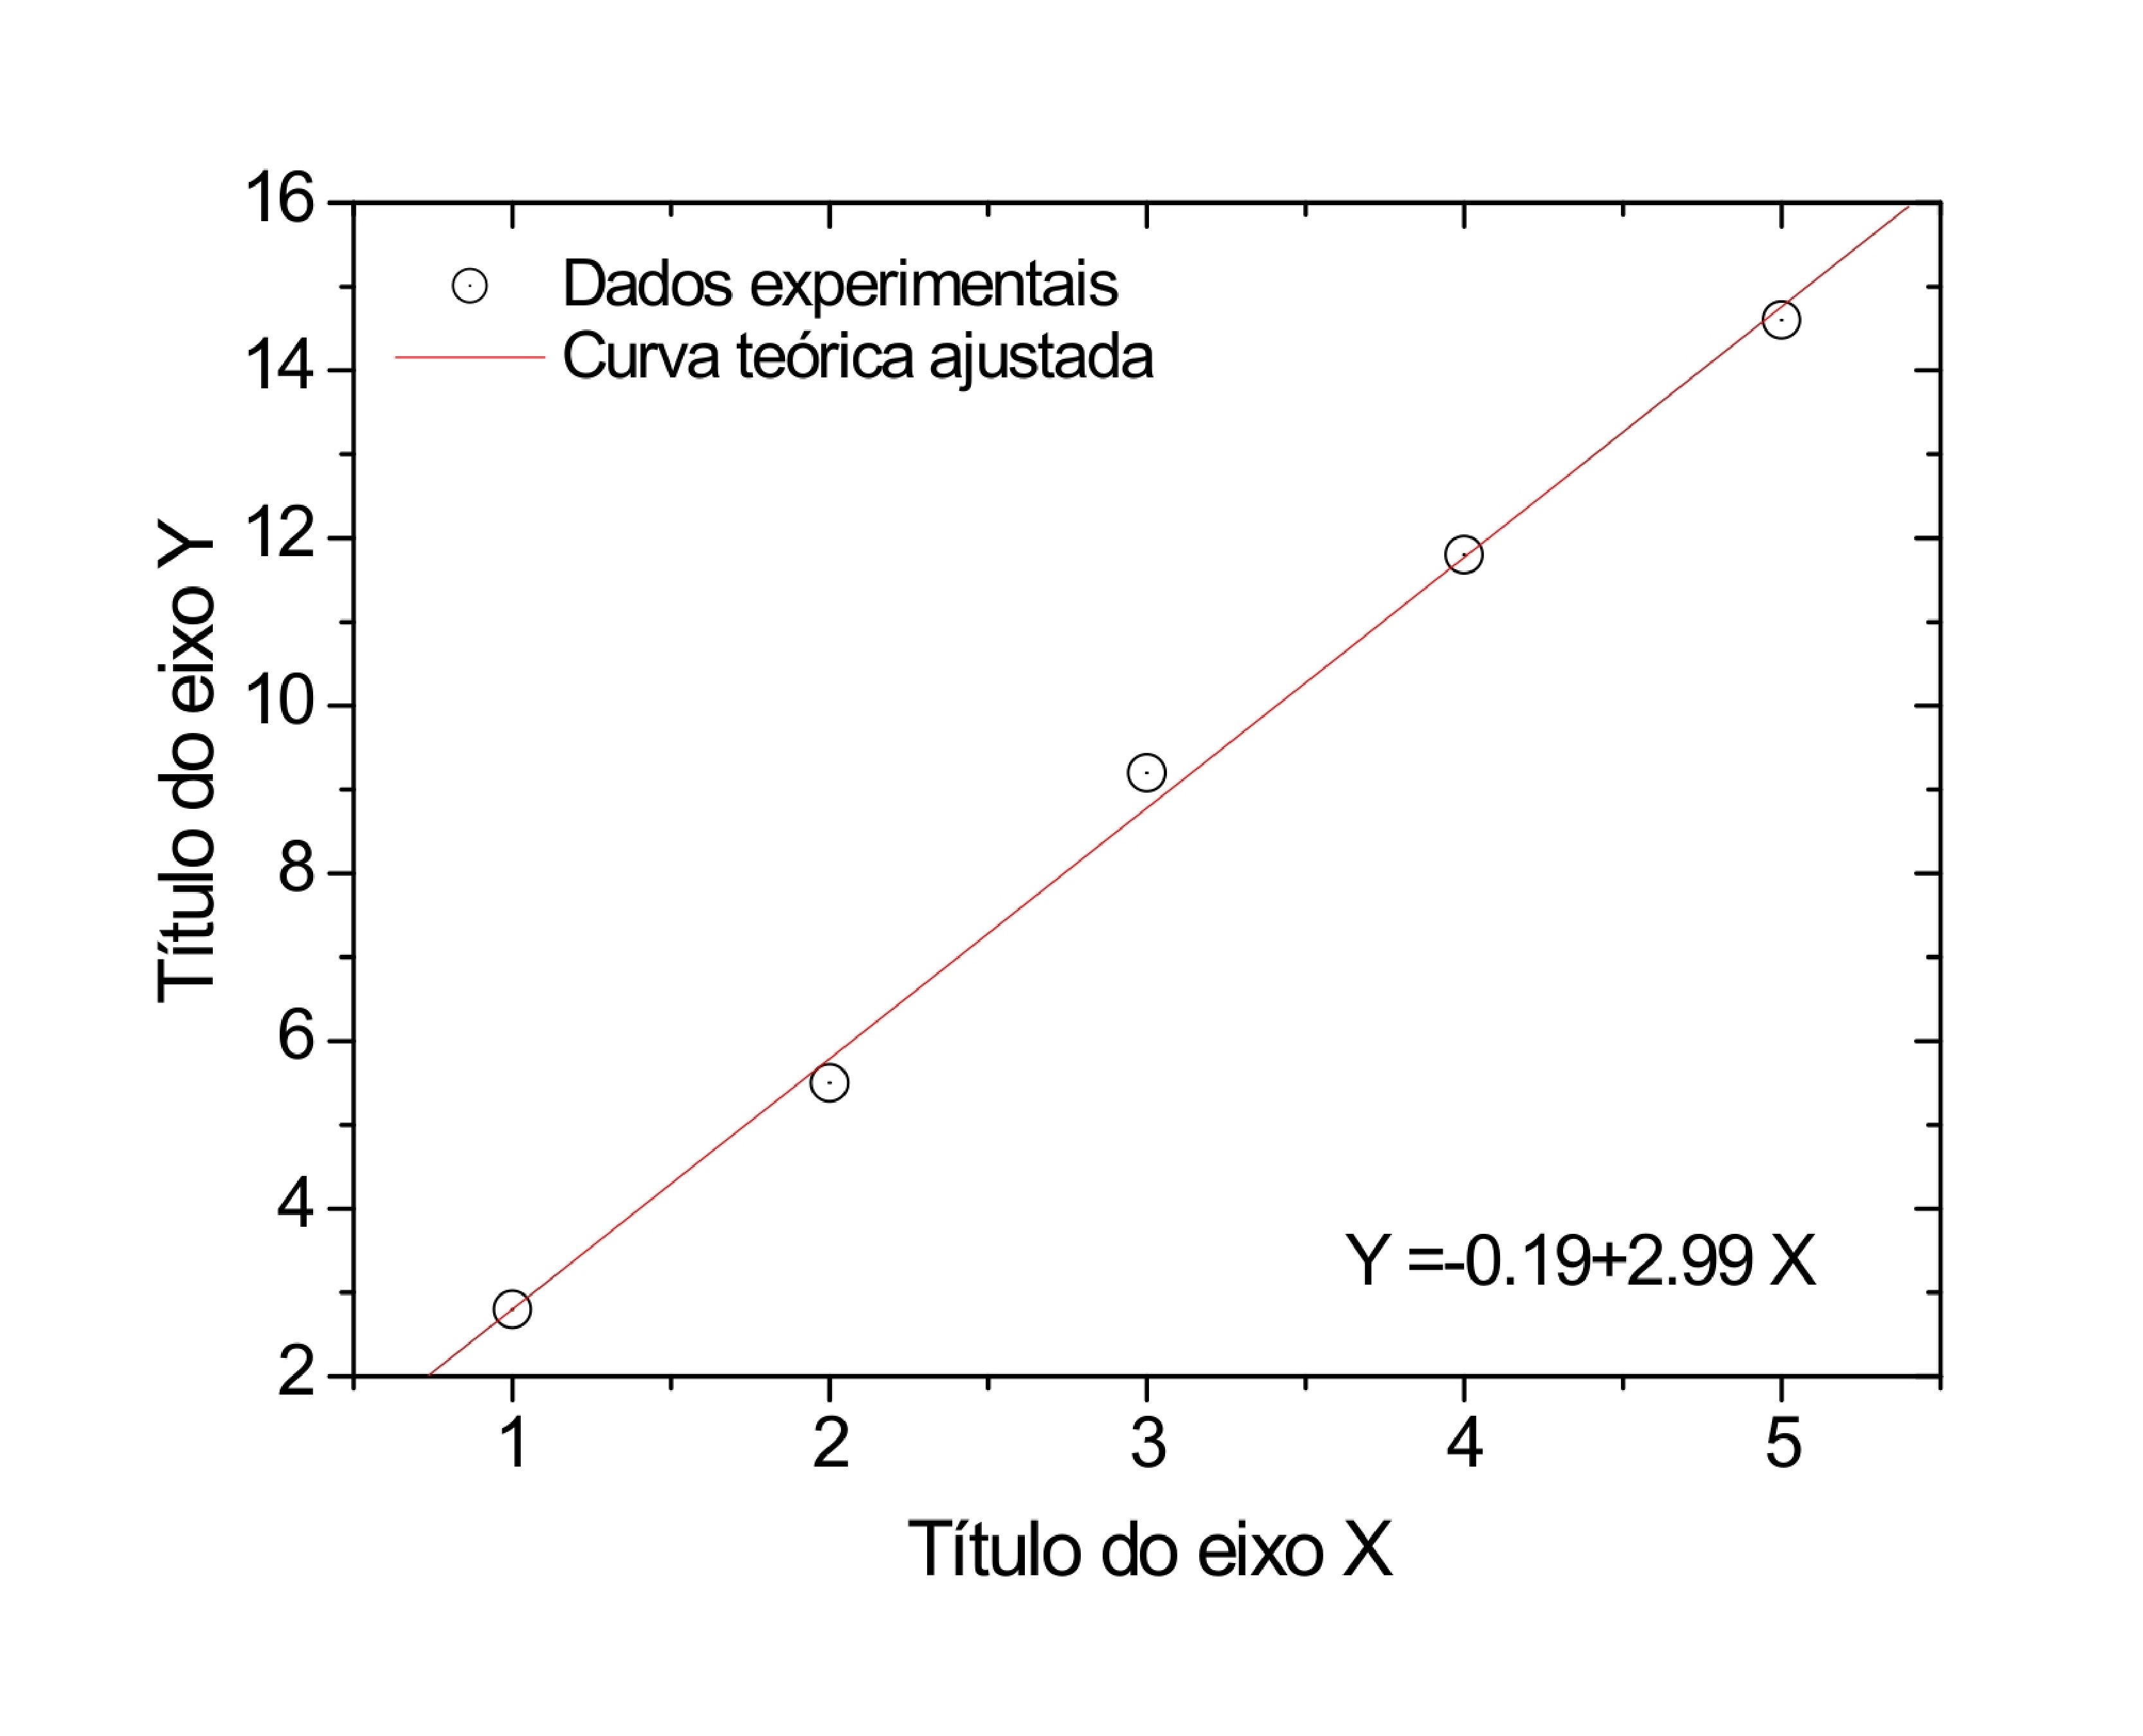
\includegraphics[keepaspectratio, width = 8.25cm]{Regressao_linear.eps}
	\caption{Esta figura é apenas um exemplo. A legenda deve vir após a figura.}
	\label{Fig_Regressao}
\end{figure}

Bem vamos a alguns detalhes. Primeiramente é recomendável que a figura esteja em um arquivo separado. O melhor formato de arquivo é o .pdf. Entretanto arquivos .eps (utilizado neste template), .jpeg e .png também funcionam. 

Apenas para fins de organização, costuma-se definir um subdiretório para armazenas os arquivos de imagem separadamente. Neste caso basta informar no arquivo .tex o diretório com o comando \verb|\graphicspath{{Figuras/}}| onde ``Figuras/''\footnote{Nota-se que o diretório é separado por barra ``/'' no padrão Unix e por contra-barra ``\textbackslash'' no padrão Windows. Note que este \textit{template} utiliza deste recurso por padrão.} é o diretório onde encontram-se as imagens.

O comando \verb|\centering| centraliza a imagem na coluna. O texto inserido dentro das chaves em \verb|\caption{}| aparecerá na legenda da figura e o texto entre \verb|\label{}| será a referência da figura. As legendas das figuras e tabelas são pré formatadas no arquivo RBClatex.cls.

Neste momento gostaria de introduzir o conceito de referência do \LaTeX. Note que na Fig.~\ref{Fig_Regressao} utilizei o \verb|\label| \verb|Fig_Regressao|. Para referir-se a está figura sem citar sua numeração, pois o \LaTeX numera automaticamente as figuras, refira-se a uam figura pelo seu \verb|label| da forma \verb|Fig.~\ref{Fig_Regressao}|. Neste caso, o comando \verb|\ref{Fig_Regressao}| é substituido pelo número da figura e o ``\textasciitilde{}'' evita que a linha seja quebrada entre o ``Fig.'' e o número.

No comando \verb|\includegraphics[]{}| entre as chaves coloque o nome do arquivo e entre os colchetes as configurações. O básico para inserir figuras sem errar é utilizar os comandos \verb|[keepaspectratio, width = 8.25cm]| que mantém a proposrção da figura com largura de 8,25~cm que é a largura da coluna.

Vou citar mais duas opções que considero úteis, a primeira é \verb|trim = 1mm 2mm 3mm 4mm,clip=true| que realiza um corte na imagem de 1, 2, 3 e 4~mm respectivamente nas margens esquerda, inferiro, direita e superior\footnote{Este corte pode ser útil para retitar bordas em branco sem ter que utilizar um editor de imagem.}. A segunda é \verb|angle=90| que rotaciona a imagem no sentido anti-horário.

Por fim vou referir-me \textit{frag} de posicionamento que fica entre os colchetes logo após \verb|\begin{figure}|. Esta \textit{flag} indica para o \LaTeX onde prefere que a figura (ou tabela) se posicione. A Tab.~\ref{Tab:Flags_Floats} indica as \textit{flags} e suas funções. para o caso dete \textit{templete}, a opção que substitui o \verb|H|\footnote{Ainda voi descobrir porque não consegui incluí-lo no RBClatex.cls. Está dando um erro que ainda não tive tempo de saná-lo.} é \verb|[!htb]|.

\begin{table}[!htb]
	\centering
	\caption{Tabela com a descrição das \textit{flags} de posicionamento. Complementei esta legenda para mostrar que o texto fica justificado.}
	\label{Tab:Flags_Floats}
	\begin{tabular}{|C{1cm}|L{7cm}|}
		\hline
		Flag & Permissão                                                                              \\ \hline
		h    & Insere a figura aproximadamente no mesmo ponto (\textit{here}) do código(pode variar um pouco). \\ \hline
		t    & Insere a figura no topo (\textit{top}) da página.                                               \\ \hline
		b    & Insere a figura na base (\textit{botton}) da página.                                            \\ \hline
		p    & Insere a figura em uma página separada.                                                \\ \hline
		!    & Substitui os parâmetros internos para forçar um determinado flag.                      \\ \hline
		H    & \textbf{Não disponível} - Coloca a figura precisamente na posição escolhida. Necessita do pacote float (\verb|\usepackage{float}|).                                      \\ \hline 
	\end{tabular}
\end{table}

Por fim, para incluir uma figura que ocupe duas colunas basta inserir um asterisco no comando, da forma \verb|\begin{figure*}[!tb]|. Utilize a \textit{flag} de posicionamento posicionar na parte superior ou na parte inferior da página. Recomenda-se, neste caso, largura máxima de 16,5~cm. Caso deseje especificar a altura da imagem sem alterar as proporções utilize \verb|[keepaspectratio, height = 4cm]|.

Os gráficos podem ser em cores. Por favor, use apenas cores sólidas as quais contrastam bem na tela e em uma via impressa em preto-e-branco, como mostrado na Fig. \ref{Fig_Regressao}. Verifique se a resolução é suficiente para revelar os detalhes importantes na figura. A Fig. \ref{Fig_Regressao} é apenas um exemplo de um gráfico experimental onde se foi ajustado uma curva teórica.

Verifique todas as figuras do artigo tanto na tela quanto em uma via impressa em preto-e-branco. Quando você verificar o seu artigo em uma via impressa em preto-e-branco, certifique-se que:
\begin{itemize} [noitemsep,topsep=0pt,leftmargin=*,labelindent=7.5mm,labelsep=2mm]
	\item as cores usadas em cada figura contrastam bem;
	\item a imagem usada em cada figura é clara;
	\item todos os rótulos de texto em cada figura são legíveis.
\end{itemize}

\subsection{Tabelas}

Assim como para figuras, mencionar as tabelas no texto como ``Tab. \ref{Tab:Flags_Floats}'' ou, se no início de uma frase, como ``Tabela \ref{Tab:Flags_Floats}''. A seguir vou apresentar algumas técnicas para tabelas, apenas o básico. Para tabelas, mais elaboradas recomento utilizar a ferramenta online https://tablesgenerator.com/.

Uma tabela é definida pelos comandos
\begin{lstlisting}
\begin{table}[!htb]
\centering
\caption{}
\label{}
\begin{tabular}{}
...
\end{tabular}
\end{table}
\end{lstlisting}

Assim como para as figuras, os comandos \verb|\centering|, \verb|\caption{}| e \verb|\label{}| exercerão as mesmas funções.

Entre os comandos \verb|\begin{tabular}{}| e \verb|\end{tabular}| devem ser inseridos os dados da tabela. Os elementos da mesma linha e de colunas diferentes são separados pelo sinal de \verb|&|. As linhas são separadas \verb|\textbackslash\textbackslash|. Para inserir uma linha separadora antes de uma linha utilize \verb|\hline|.

Nos colchetes do comando \verb|\begin{tabular}{}| é possível especificar as linhas verticais e o alinhamento das colunas. Por exemplo, tres colunas alinhadas respectivamente a esquerda, centro e direita são especificadas da forma \verb|{ lcr}|. Neste caso a largura é determinada pelo conteúdo como indicado na Tab.~\ref{Tab:Exemplo1} e a linha vertical por uma barra vertical ``\textbar''. 

Se desejar especificar a largura das colunas, utilize \verb|{L{1cm}C{1cm}R{1cm}|, como apresentado na Tab.~\ref{Tab:Exemplo2}. Lembrando que o espaçamento entre colunas é de 0,5~mm e a largura da coluna é 8,25~mm.

\begin{table}[!htb]
	\centering
	\caption{Exemplo de tabela utilizando ``lcr''}
	\label{Tab:Exemplo1}
	\begin{tabular}{|lcr|}
		\hline
		(1,1) & (1,2) & (1,3) \\ 
		(2,1) & (2,2) & (2,3) \\ 
		(3,1) & (3,2) & (3,3) \\ \hline
	\end{tabular}
\end{table}

\begin{table}[!htb]
	\centering
	\caption{Exemplo de tabela utilizando ``L\{1cm\}C\{1cm\}R\{1cm\}''.}
	\label{Tab:Exemplo2}
	\begin{tabular}{|L{1cm}C{1cm}R{1cm}|}
		\hline
		(1,1) & (1,2) & (1,3) \\
		(2,1) & (2,2) & (2,3) \\
		(3,1) & (3,2) & (3,3) \\ \hline
	\end{tabular}
\end{table}

Nas duas tabelas o conteúdo entre os comandos \verb|\begin{tabular}{}| e \verb|\end{tabular}| são:
\begin{lstlisting}
\hline
(1,1) & (1,2) & (1,3) \\
(2,1) & (2,2) & (2,3) \\
(3,1) & (3,2) & (3,3) \\ \hline
\end{lstlisting}.

Por fim, assim como para figura, para incluir uma tabela que ocupe duas colunas basta inserir um asterisco no comando, da forma \verb|\begin{table*}[!tb]|. 

\section{Referências}

Nesta parte temos algumas vantagens e desvantagens de utilizar o \LaTeX. Na humilde opinião deste autor são muito mais vantagens. Nesta seção não detalharemos o sistema de referência em \LaTeX. O objetivo é apenas informar uma forma pratica de organizá-las para a Revista Brasileira de Criminalística. As formatações da lista de referências são feitas automaticamente em ordem de apresentação no texto pelo arquivo de estilos ``RBC.bst''. Primeiramente será explicado como organizar suas referências e em seguida como citá-las ao longo do texto.

Uma forma de utilizar referências em \LaTeX é organizá-las em um arquivo separado com a extensão .bib. Este arquivo é referenciado no .tex como comando \verb|\bibliography{Modelo_RBC_latex}| que deve ser inserido antes dos apêndices ou anexos.

Neste arquivo cada tipo de referência (artigo, livro, tese, etc...) possui um formato. Existem vários \textit{softwares} para gerenciar referências em \LaTeX, particularmente recomendamos o Jabref\footnote{Que pode ser obtido gratuitamente em: http://www.jabref.org/}. O \textit{template} original descreve como referenciar Artigos de revistas, Artigos encaminhados para publicação, Dissertações, Teses, Livros e Páginas da web. Neste \textit{template} tomei a liberdade de incluir referências a capítulo de livro. %, procedimento operacional padrão(POP) e laudo pericial.

\subsection{Artigos}

Um artigo é inserido no arquivo .bib da forma:
\begin{lstlisting}
@Article{Chave_Citacao,
Title	= {},
Author = {},
Journal = {},
Year = {},
Volume = {},
Number = {},
Pages = {},
Month = {}, 
Note = {},
Key = {},
Doi = {} }
\end{lstlisting}

Os campos \verb|Chave_Citacao|, \verb|Title|, \verb|Author|, \verb|Journal| e \verb|Year| são obrigatórios.

A chave de citação é como o artigo é referenciado ao longo do texto. Sobre o uso de caracteres especiais, e.g. acentos e cedilhas, utilize os \textit{Escaped codes}\footnote{Tabela dos códigos disponíveis em https://en.wikibooks.org/wiki/LaTeX/Special\_Characters.}. Se desejar colocar uma sigla toda maiúscula utilize colchetes. para o nome do autor entre com o sobrenome de citação separado por vírgula. Em caso de mais de um autor separe com o \verb|and|. As referências \cite{Gold2011,Dias2011,Silva2017,Pires2005} são os respectivos exemplos de artigo, artigo encaminhado para publicação e artigo em anais de congresso.

Por exemplo:
\begin{lstlisting}
@Article{Dias2011,
Title	= {Comori{\^e}ncia: pondera{\c{c}}{\~o}es 
jur{\'\i}dicas e tanatol{\'o}gicas},
Author = {Dias, CR and Antedomenico, E},
Journal = {Rev. Tribunais},
Year = {2011} }
\end{lstlisting}

Se for um artigo encaminhado para publicação troque o campo \verb|Year| para \verb|{Para ser publicado em 2011}|. Se for um artigo em anais de congresso troque o tipo \verb|@Article| por \verb|@InProceedings|, e \verb|Journal| por \verb|BookTitle|. Neste último insira o título dos anais do congresso.

\subsection{Livro e capítulo de livro}

Uma referência do tipo livro possui a seguinte formatação:
\begin{lstlisting}
@Book{Fricke1990,
Title = {Traffic accident reconstruction},
Author = {Fricke, Lynn B},
Publisher = {Northwestern University Traffic Institute},
Year = {1990},
Note = {210-234} }
\end{lstlisting}

O campo \verb|Publisher| é para editora e \verb|Note| foi reservado para indicar as páginas consultadas. Caso o livro seja uma coleção de vários autores onde um editor que realizou a coleção altere o campo \verb|Author| por \verb|Editor|, por exemplo: 
\begin{lstlisting}
@book{casey2001,
Title={Handbook of computer crime investigation: 
forensic tools and technology},
Editor={Casey, Eoghan},
Year={2001},
Publisher={Elsevier} }
\end{lstlisting}

Em caso de capítulo de livro troque o tipo \verb|@Book| por \verb|@InCollection| como no exemplo:
\begin{lstlisting}
@InCollection{Amino2012,
Title = {Historical and procedural overview 
of forensic speaker recognition as a 
science},
Editor={Neustein, Amy and Patil, Hemant A},
Author = {Amino, Kanae and Osanai, Takashi 
and Kamada, Toshiaki and Makinae, Hisanori 
and Arai, Takayuki},
Booktitle = {Forensic speaker recognition},
Year = {2012},
Publisher = {Springer},
Pages = {3--20} }
\end{lstlisting}

Estes exemplos aparecem citados em \cite{Fricke1990,Casey2001,Amino2012}. 

\subsection{Teses e dissertações}

Teses e dissertações são inseridas utilizando respectivamente os comandos \verb|@PhdThesis| e \verb|@MastersThesis| como nas referências \cite{ABEL2001,Silva2007}. A seguir tem-se um exemplo do código.

\begin{lstlisting}
@PhdThesis{ABEL2001,
Title = {Estudo da Per{\'\i}cia em 
Petrografia Sedimentar e sua 
Import{\^a}ncia para a Engenharia 
de Conhecimento},
Author = {Mara Abel},
School = {Departamento de Engenharia 
Civil, Universidade Federal do Rio 
Grande do Sul},
Year = {2001} }
\end{lstlisting} 

\subsection{Páginas da web}

Páginas da web, devem conter nome(s) do(s) autor(es), abreviação do periódico, número do volume, número da página, ano da publicação, data de consulta e o sítio da internet onde se encontra. Utilize o tipo \verb|@Misc| e o campo \verb|Note| para indicar o sitio da internete e data de acesso. Veja exemplo em \cite{DeMoore1999a} exemplificado a seguir.

\begin{lstlisting}
@Misc{DeMoore1999a,
Title = {Suicide attempts...},
Author = {De Moore, G. M. 
and Robertson, A. R.},
Note = {Retirado em 01/01/2011, 
de http://www.xxx.com.br},
Year = {1999},
Journal = {American journal of psychiatry},
Number = {9},
Pages = {1425--1431},
Publisher = {Am Psychiatric Assoc},
Volume = {156} }
\end{lstlisting}

\subsection{Citações}

Ao se referir a um item da referência, por favor, basta utilizar o a chave da referência com comando \verb|\cite{}|. Por exemplo \verb|\cite{Silva2007}| vai gerar a numeração da referência entre colchetes. Não use ``Ref.~\cite{ABEL2001}'' ou ``Referência~\cite{ABEL2001}'', exceto no início de uma frase, por exemplo, ``Referência~\cite{ABEL2001} mostra...'' (em código: \verb|``Referência~\cite{ABEL2001} mostra...''|). 

Várias referências são numeradas com suportes distintos (por exemplo, \cite{Silva2007}, \cite{Pires2005, Fricke1990,Dias2011}). 

Por fim gostaria de apresentar uma forma de obter o código de uma referência de forma mais amigável. O Google Acadêmico\footnote{https://scholar.google.com.br/} oferece a opção de citar para os resultados de suas buscas. Desta forma é possível obter o código Bib\TeX clicando no caminho ``citar'' do artigo e em seguida em ``BibTex'', como indicado pelas setas na Fig.\ref{Fig:Google_Academico}.

\begin{figure}[h]
	\centering
	\includegraphics[keepaspectratio, width = 8.25cm]{Google_Academico.pdf}
	\caption{Captura de tela indicando os caminhos para obter o código de uma referência em Bib\TeX.}
	\label{Fig:Google_Academico}
\end{figure} 

\section{Modo matemático, equações e teoremas}

O \LaTeX possui um ferramental extremamente refinado para apresentação de expressões matemáticas e equações. O modo matemático permite inserir texto sobrescrito, subscrito, letras gregas e outros símbolos\footnote{Uma boa lista de símbolos em \LaTeX pode ser consultada em https://en.wikipedia.org/wiki/Wikipedia:LaTeX\_symbols}. 

Para entrar no modo matemático ao longo do texto utilize o \$ para delimitar o trecho, desta forma a expressão $2\pi\vec{v}$ possui código \verb|$2\pi\vec{v}$|.

Assim como as figuras e tabelas, as equações são numeradas automaticamente e inseridas entre os comandos de \verb|\begin{equation}| e \verb|end{equation}| da forma:
\begin{lstlisting}
\begin{equation} \label{Eq:Calculo}
\int\limits_{x=a}^{x=b}f'(x)dx = f(b)-f(a).
\end{equation}
\end{lstlisting}
sendo apresentada na Eq.~\ref{Eq:Calculo} a seguir
\begin{equation} \label{Eq:Calculo}
\int\limits_{x = a}^{x=b} f'(x)dx = f(b) - f(a).
\end{equation}

Mencionar as equações no texto como “Eq.~\ref{Eq:Calculo}” (código \verb|Eq.~\ref{Eq:Calculo}|) ou, se no início de uma frase, como “Equação~\ref{Eq:Calculo}”.

O modo matemático do \LaTeX possui muito recursos. Se preferir utilizar um editor de equações os autores sugerem https://www.latex4technics.com/.

% ---
% Finaliza a parte no bookmark do PDF, para que se inicie o bookmark na raiz
% ---
%\bookmarksetup{startatroot}% 
% ---

% ---
% Conclusão
% ---
\section{Conclusões}
\addcontentsline{toc}{section}{Conclusões}

A versão deste modelo é V1. Qualquer dúvida a respeito do modelo apresentado entre em contato com a Revista.

\section*{Agradecimentos}
\addcontentsline{toc}{section}{Agradecimentos}

A Revista Brasileira de Criminalística gostaria de agradecer aos Peritos Criminais participantes que se dispuseram a tirar a revista do campo das ideias e materializá-la, bem como a Associação Brasileira de Criminalística – ABC pelo apoio concedido.
%
%blabla
%
%blabla
% ----------------------------------------------------------
% ELEMENTOS PÓS-TEXTUAIS
% ----------------------------------------------------------
%\postextual


%]  				% FIM DE ARTIGO EM DUAS COLUNAS
% ---

% ----------------------------------------------------------
% Referências bibliográficas
% ----------------------------------------------------------
\bibliography{Modelo_RBC_latex}

% ----------------------------------------------------------
% Glossário
% ----------------------------------------------------------
%
% Há diversas soluções prontas para glossário em LaTeX. 
% Consulte o manual do abnTeX2 para obter sugestões.
%
%\glossary

% ----------------------------------------------------------
% Apêndices
% ----------------------------------------------------------

\section*{Apêndices ou anexos}

Revista Brasileira de Criminalística sugere utilizar apêndices ou anexos somente em último caso. Entretanto, se for necessário, esta seção virá após as Referências Bibliográficas.

Considera-se apêndice o texto ou documento elaborado pelo autor, a fim de complementar sua argumentação, sem prejuízo da unidade nuclear do trabalho. Considera-se anexo o texto ou documento não elaborado pelo autor, que serve de fundamentação, comprovação e ilustração.


\end{document}
